% !TeX root = ../main.tex
\chapter{Planificación}
\label{cap:planificacion}

Para conseguir un correcto desarrollo del proyecto es necesario establecer una planificación detallada que organice las distintas fases del trabajo a lo largo del curso.

El TFG de Ingeniería Multimedia en la Universidad de Alicante corresponde a 12 créditos ECTS, es decir, 300 horas de trabajo. El proyecto se plantea desde septiembre de 2026 con la defensa como horizonte en mayo de 2027, lo que deja nueve meses para repartir la carga de forma progresiva. Además, debe compaginarse con el resto de asignaturas del curso, las prácticas y otros trabajos puntuales, por lo que la planificación se ha diseñado con cierto margen para absorber estas cargas adicionales sin comprometer los plazos de
entrega.

La naturaleza del proyecto condiciona el reparto de horas. VH SimGrid no es solo una aplicación de escritorio: incluye tres periféricos físicos (el volante de \textit{force feedback} VH Grid DD15, la pedalera VH Axis y el aro VH Formula Apex), cada uno con su propio firmware, y una aplicación que los configura en vivo y añade dash, ingeniero de pista por voz y análisis de telemetría. Por ello, la fase de implementación y evaluación concentra la mayor parte del esfuerzo, y las pruebas se realizan sobre el hardware real y con
simuladores comerciales.

Siguiendo la metodología DSR descrita en el capítulo anterior, la planificación temporal se organiza en torno a sus fases principales, complementadas con el uso de un tablero Kanban para la gestión diaria del trabajo.

\begin{table}[H]
	\centering
	\renewcommand{\arraystretch}{2}
	\begin{tabular}{|l|p{4cm}|l|}
		\hline
		\textbf{Fase} & \textbf{Duración estimada} & \textbf{Fecha límite} \\
		\hline
		Identificación del problema y objetivos & 40 horas & 31/10/2026 \\
		\hline
		Diseño y desarrollo de la solución & 55 horas & 31/12/2026 \\
		\hline
		Implementación y evaluación & 140 horas & 15/04/2027 \\
		\hline
		Comunicación & 65 horas & 31/05/2027 \\
		\hline
		\textbf{Total} & \textbf{300 horas} & \\
		\hline
	\end{tabular}
	\caption{Planificación temporal resumida del TFG}
	\label{tab:planificacion}
\end{table}

A continuación se describe el contenido de cada fase:

\begin{itemize}
	\item \textbf{Identificación del problema y objetivos (40 h).} Planificación
	del trabajo, introducción y propuesta de solución, definición de objetivos, elección de la metodología y estudio del estado del arte: periféricos comerciales de simracing, proyectos DIY de \textit{force feedback} y software de configuración, dashes y telemetría existente.
	
	\item \textbf{Diseño y desarrollo de la solución (55 h).} Análisis y especificación de requisitos de los periféricos y de la aplicación, y diseño del sistema: arquitectura hardware (controladora del motor, electrónica de la pedalera y del aro), protocolo de comunicación entre firmware y aplicación, arquitectura de la aplicación y diseño de su interfaz.
	
	\item \textbf{Implementación y evaluación (140 h).} Desarrollo de los tres firmwares (FFB nativo por USB HID PID en el volante, lectura de sensores Hall y célula de carga en la pedalera, LEDs, botones y encoders en el aro), de la aplicación de configuración en vivo, de las funciones de telemetría (dash, ingeniero de pista y análisis) y su documentación. Se cierra con las pruebas
	y la validación sobre hardware real y en los simuladores compatibles, incluida la evaluación de las protecciones de seguridad del volante.
	
	\item \textbf{Comunicación (65 h).} Redacción final de la memoria
	(resumen, motivación, resultados, conclusiones y trabajo futuro), revisión de bibliografía y glosario, y preparación de la defensa del TFG en mayo de 2027.
\end{itemize}

Para complementar esta visión, en la sección~\ref{sec:gantt} se presenta un diagrama de Gantt que muestra de forma gráfica las fases del proyecto y sus duraciones, detallando las tareas en las que se ha dividido cada una de ellas.

% ---------- Página en horizontal para el Gantt ----------
\newpage
\begin{landscape}
	\thispagestyle{empty}
	\section{Diagrama de Gantt}
	\label{sec:gantt}
	\begin{figure}[H]
		\centering
		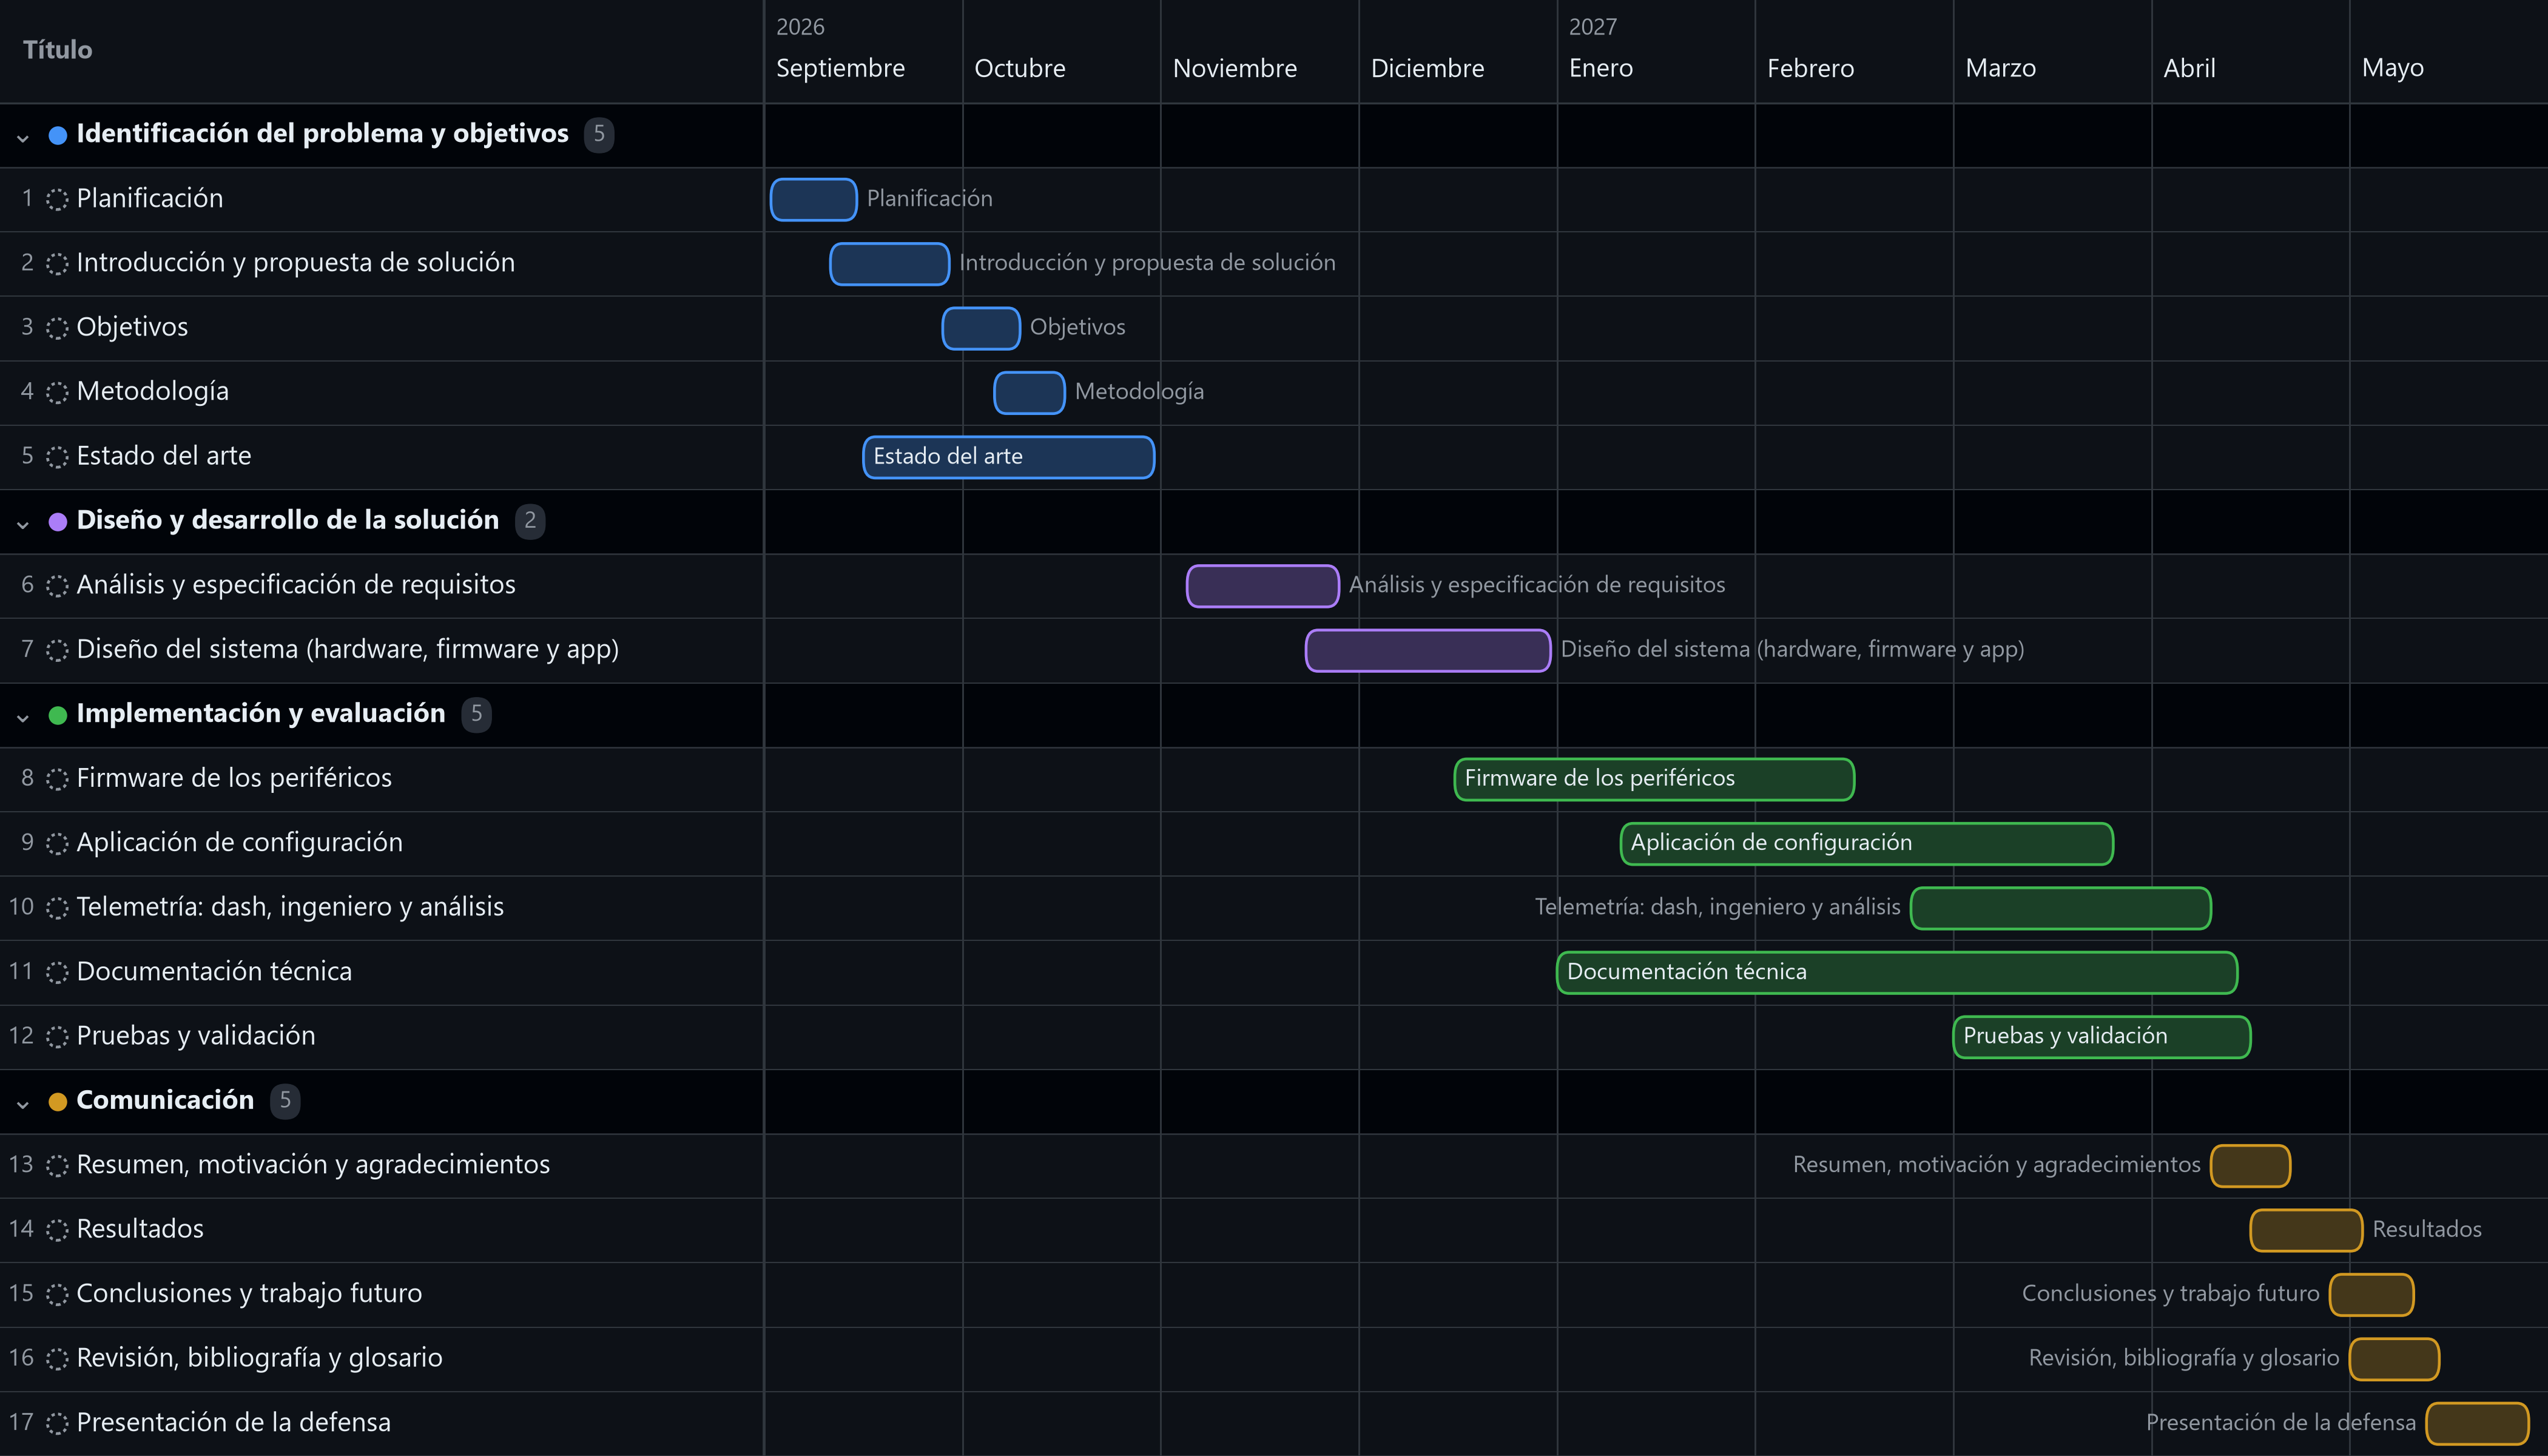
\includegraphics[width=\linewidth, height=0.8\textheight, keepaspectratio]{img/gantt_github.png}
		\caption[Diagrama de Gantt]{Diagrama de Gantt. (Fuente propia)}
		\label{fig:gantt}
	\end{figure}
\end{landscape}